\chapter[Contextualização]{Contextualização}

Competições universitárias de foguetes são eventos em que equipes formadas por estudantes (de engenharia, em sua maioria) precisam desenvolver um foguete experimental que consiga atingir uma altitude máxima específica (1km, 3km ou 7km, dependendo da competição). O propósito dessas competições é incentivar os participantes a se envolverem no desenvolvimento de um projeto desafiador e ao mesmo tempo estimulante, semelhante a eventos estudantis de nível médio ou mesmo fundamental, nos quais a propulsão do foguete é emulada com experimentos lúdicos (com o uso de bicarbonato de sódio, ou bombas de pressão)\footnote{Cf. Mostra Brasileira de Foguetes (MOBFOG): https://bit.ly/3c968ki}, porém não menos interessantes.
\par No entanto, diferente desses eventos, numa competição universitária, são utilizados propulsores a combustão, semelhantes aos utilizados em foguetes reais, ainda que em escala reduzida (por isso experimentais). Essa exigência demanda, naturalmente, uma série de medidas de seguranças que devem ser observadas pelas equipes durante as competições. Uma dessas medidas é o raio de distância mínima da base de lançamento, que define a área na qual nenhuma pessoa deve ficar durante o lançamento do foguete\footnote{Cf. Latin America Space Challenge (LASC): https://bit.ly/2FQ2Ru9}. Isso exige que alguns atos preparatórios do lançamento sejam feitos remotamente.
\par A Capital Rocket Team (CRT) é a equipe da Universidade de Brasília dedicada a participar dessas competições de foguetes. Fundada em 2015 por estudantes do curso de Engenharia Aeroespacial, desde sua origem a equipe trabalha com um tipo específico de propulsão: a propulsão híbrida. Nela, as substâncias responsáveis pela propulsão (chamadas de par propelente) são armazenadas no foguete em estados físicos distintos \cite{sutton}. No caso dos foguetes da Capital, o combustível (parafina) fica em estado sólido, em formato cilíndrico dentro da câmara de combustão do motor, enquanto o oxidante (óxido nitroso) fica em estado líquido em um tanque separado.
\par O sistema propulsivo é completado por um ignitor, que fica junto ao combustível na câmara de combustão, uma substância que necessita somente de uma fonte de calor (que pode ser um resistor elétrico) para iniciar sua combustão. Na hora do lançamento, uma corrente elétrica aquece o resistor. O tanque contendo o óxido nitroso é aberto, despejando o oxidante na câmara de combustão. A mistura do oxidante com o combustível contido na câmara, mais o calor gerado pela combustão do ignitor, provoca a reação principal de combustão do propulsor. Os gases resultantes dessa combustão são expelidos pelo bocal de saída do motor (chamado de tubeira). Essa saída dos gases gera uma força de empuxo direcionada para o solo, o que faz o foguete deslocar no sentido oposto, em direção ao apogeu. E assim é feita a decolagem do foguete.

\section{Problematização}

Como visto, as características de um foguete de propulsão híbrida, somadas com as exigências de segurança da competição, somadas também com as necessidades típicas de uma missão de lançamento (como o registro da altitude durante o voo) resultam em uma série de demandas que a Capital Rocket Team precisa atender para ter uma missão bem sucedida. Para fins deste trabalho, a Capital será tratada como um cliente (e referenciada por esse termo a partir de agora) que deseja contratar um serviço prestado pela presente equipe de Projeto Integrador 2 (referenciada a partir de agora como "equipe") para sanar algumas dessas demandas, as quais são:
\begin{itemize}
    \item fazer o abastecimeno do tanque de oxidante remotamente, uma vez que o foguete já esteja colocado na base de lançamento e a mangueira de abastecimento esteja acoplada a ele manualmente (o que é permitido pelas regras de segurança);
    \item fazer a ignição do foguete remotamente, a qual consiste em emitir um sinal elétrico capaz de aquecer o resistor ligado ao ignitor pelo tempo necessário para que este inicie sua combustão, bem como em abrir a válvula que conecta o tanque do oxidante ao motor do foguete;
    \item fazer a coleta dos dados de telemetria do foguete durante o voo, de modo a registrar tanto sua variação de altitude e velocidade em tempo real como sua posterior localização, para fins de recuperação.
\end{itemize}
\par Essas demandas possuem o elemento comum de serem, de uma forma ou de outra, a execução de uma tarefa à distância. Ademais, cada uma delas tem características específicas que são variáveis conforme as dimensões do foguete. Por exemplo, a quantidade de oxidante necessária para o tanque do foguete varia conforme a altitude de apogeu desejada (quanto maior o apogeu, maior o tempo de voo e, consequentemente, maior será a quantidade necessária de oxidante para a combustão).
\par Para fins do presente projeto, a equipe utilizar-se-á dos parâmetros com que o cliente trabalha atualmente (foguete de apogeu de 1km). No entanto, a solução a ser desenvolvida precisará observar esse caráter variável de alguns parâmetros presentes nas demandas contidas na execução de uma missão de lançamento.
\par A proposta da equipe é o desenvolvimento de uma estação de controle remota capaz de coordenar essas diversas atividades, por meio do envio e recebimento de sinais que sejam capazes de coletar os dados pertinentes à operação de lançamento e ao voo subsequente, bem como atuar sobre dispositivos que executem as tarefas demandadas (como por exemplo a abertura ou fechamento de válvulas).

\begin{figure}[H]
\centering
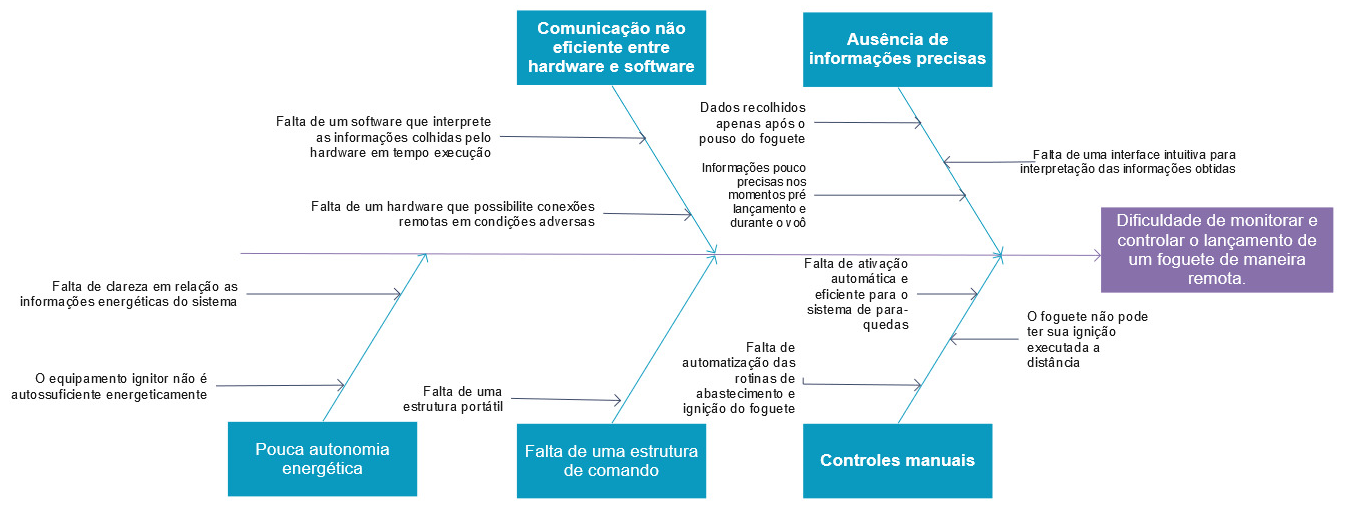
\includegraphics[width=\textwidth]{figuras/Fishbone}
\caption{\textit{Fishbone}}
\label{fig:fishbone}
\end{figure}

\section{Justificativa}

Há dois pontos que precisam ser fundamentados a respeito do projeto: a escolha da demanda e a natureza da solução proposta para essa demanda. Quanto à escolha da demanda, optou-se por atender um problema concreto enfrentado por um agente que atua efetivamente na área de tecnologia. Ainda que o propósito principal da equipe seja de fato atender as diretrizes estabelecidas pela matéria, adotar um \textit{stakeholder} adicional traz a dupla vantagem de: a) definir requisitos do projeto de maneira clara, uma vez que o que se precisa ou não fazer é expresso pelo trabalho que o cliente já desenvolve; e b) dar destinação útil ao projeto (caso aprovado) após o fim da matéria, o que está em consonância com o propósito do curso de promover o desenvolvimento de produtos que tenham aplicação prática e/ou potencialmente comercial.
\par Quanto à natureza da solução, acreditamos que o projeto está voltado a tornar uma rotina de trabalho mais eficiente e segura. Como vimos nos requisitos de segurança das competições, uma plataforma que automatize uma série de tarefas necessárias para a preparação do lançamento de um foguete é mais do que bem-vinda, em favor da segurança dos membros de uma equipe de competição. Ademais, o cliente já reportou dificuldades passadas quanto a essas tarefas, em particular o abastecimento do tanque e o desacoplamento da mangueira, feitos com um sistema de cordas e polias em caráter contingencial. \par Desenvolver uma solução definitiva para essas atividades acessórias permitirá que o cliente torne mais produtivo seu trabalho voltado especificamente no desenvolvimento do seu foguete e, quem sabe, o trabalho de outras equipes interessadas e que atuem em projetos semelhantes, o que, em última análise, ajudará no desenvolvimento da atividade espacial brasileira como um todo.